\documentclass[dutch]{ucll-slides}
\usepackage{pxfonts}
\usepackage{tikz}
\usepackage{calc}
\usepackage{ucll-code}
\usepackage{siunitx}


\usetikzlibrary{calc,shadows,tikzmark}

\coursename{Scripttalen}
\title{Hashing}



\begin{document}

\maketitle

\begin{frame}
  \frametitle{Premisse}
  \begin{itemize}
    \item Je bewaakt toegang tot een gebouw
    \item Je hebt een lijst namen
    \item Enkel mensen op de lijst mogen binnen
    \item Dit moet zo effici\"ent mogelijk gebeuren
  \end{itemize}
\end{frame}

\begin{frame}
  \frametitle{Korte Lijsten}
  \begin{center}
    \begin{tabular}{rl}
      $\square$ & Jan \\
      $\square$ & Pieter \\
      $\square$ & Dorien \\
      $\square$ & Eric \\
    \end{tabular}
  \end{center}
  \begin{itemize}
    \item Namen in random volgorde
    \item Ok indien klein aantal namen
  \end{itemize}
\end{frame}

\begin{frame}
  \frametitle{Lineair Zoeken}
  \begin{columns}
    \column{4cm}
    \begin{center}
      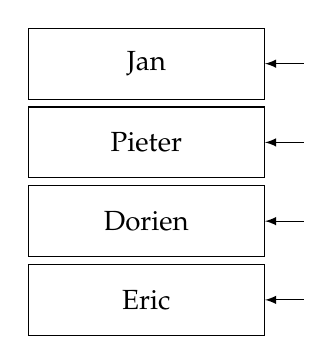
\begin{tikzpicture}
        \foreach[count=\i] \name in {Jan,Pieter,Dorien,Eric} {
          \node[anchor=south west,draw,minimum width=3cm,minimum height=0.9cm] (name \i) at (0,-\i) {\name};
        }
        
        \foreach[evaluate={int(\i+1)} as \j] \i in {1,...,4} {
          \visible<\j>{
            \draw[latex-] (name \i.east) -- ++(0.5,0);
          }
        }
      \end{tikzpicture}
    \end{center}

    \column{6cm}
    \code[language=python,width=\linewidth]{linear-search.py}
  \end{columns}
  \vskip5mm
  \begin{itemize}
    \item Zoeken naar naam vergt lijst afgaan
    \item Bv.~zoeken naar Eric $\rightarrow$ 4 vergelijkingen nodig
  \end{itemize}
\end{frame}

\begin{frame}
  \frametitle{Verbetering}
  \begin{center}
    \begin{tabular}{rlrlrl}
      $\square$ & An      & $\square$ & Gunther   & $\square$ & Mieke \\
      $\square$ & Bart    & $\square$ & Hannelore & $\square$ & Nadia \\
      $\square$ & Dorien  & $\square$ & Idriss    & $\square$ & Patrick \\
      $\square$ & Eric    & $\square$ & Jolien    & $\square$ & Sanne \\
      $\square$ & Frans   & $\square$ & Karel     & $\square$ & Thomas \\
    \end{tabular}
  \end{center}
  \begin{itemize}
    \item Voor grotere aantallen is betere organisatie nodig
    \item Alfabetisch sorteren versnelt het proces
  \end{itemize}
\end{frame}

\begin{frame}
  \frametitle{Binair Zoeken}
  \begin{center}
    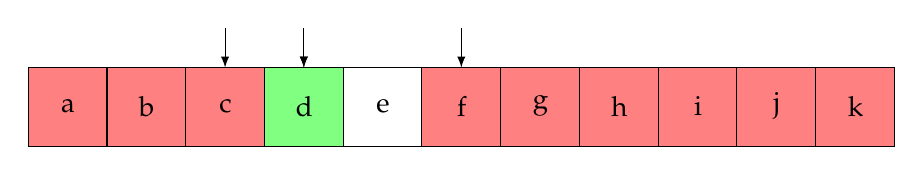
\begin{tikzpicture}[u/.style={fill=white},m/.style={fill=red!50},f/.style={fill=green!50}]
      \visible<1>{
        \foreach[count=\i] \x in {u,u,u,u,u,u,u,u,u,u,u} {
          \draw[\x] (\i,0) rectangle ++(1,1);
        }
      }

      \visible<2>{
        \foreach[count=\i] \x in {u,u,u,u,u,u,u,u,u,u,u} {
          \draw[\x] (\i,0) rectangle ++(1,1);
        }
        \draw[latex-] (6.5,1) -- ++(0,0.5);
      }

      \visible<3>{
        \foreach[count=\i] \x in {u,u,u,u,u,m,m,m,m,m,m} {
          \draw[\x] (\i,0) rectangle ++(1,1);
        }
        \draw[latex-] (3.5,1) -- ++(0,0.5);
      }

      \visible<4>{
        \foreach[count=\i] \x in {m,m,m,u,u,m,m,m,m,m,m} {
          \draw[\x] (\i,0) rectangle ++(1,1);
        }
        \draw[latex-] (4.5,1) -- ++(0,0.5);
      }

      \visible<5>{
        \foreach[count=\i] \x in {m,m,m,f,u,m,m,m,m,m,m} {
          \draw[\x] (\i,0) rectangle ++(1,1);
        }
        \draw[latex-] (4.5,1) -- ++(0,0.5);
      }

      \foreach[count=\i] \x in {a,b,c,d,e,f,g,h,i,j,k} {
        \node[anchor=south west,minimum size=1cm] at (\i,0) {\x};
      }
    \end{tikzpicture}
  \end{center}

  \begin{itemize}
    \item Bv. zoeken of d in de lijst zit
    \item Beginnen in het midden
    \item Elke vergelijking schrapt helft van mogelijkheden
    \item 11 namen $\rightarrow$ max.~4 vergelijkingen nodig
    \item $10^6$ namen $\rightarrow$ max.~20 vergelijkingen nodig
    \item $10^{82}$ namen $\rightarrow$ max.~273 vergelijkingen nodig
  \end{itemize}
\end{frame}

\begin{frame}
  \frametitle{Kan Het Nog Sneller?}
  \begin{itemize}
    \item Als je in een woordenboek ``zebra'' opzoekt, begin
          je dan in in het midden van het woordenboek?
    \item Je weet dat zebra ergens op 't einde zal staan
    \item Als eerste stap ``gok'' je dus waar het woord zal staan
          door het woordenboek op 't einde open te klappen
    \item Vervolgens zoek je alfabetisch
    \item Hoe kunnen we dit gokken implementeren?
  \end{itemize}
\end{frame}

\begin{frame}
  \frametitle{Poging \#1}
  \begin{itemize}
    \item Je neemt 26 bladen en nummert ze
    \item Je wil op basis van de naam meteen weten op welk blad het zal staan
    \item Je kent aan elke letter $\ell$ een uniek getal $\mathrm{ord}(\ell)$ toe
          \[
            \mathrm{ord}(a) = 0 \qquad \mathrm{ord}(b) = 1 \qquad \mathrm{ord}(c) = 2 \qquad \dots
          \]
    \item Paginanummer wordt bepaald door eerste letter
          \begin{itemize}
            \item \textbf{A}n staat op pagina 0
            \item \textbf{B}jorn op pagina 1
            \item \textbf{C}harlie op pagina 2
          \end{itemize}
    \item In code: bladen staan in array, tussen 5de blad vinden gaat in \'e\'en stap
  \end{itemize}
\end{frame}

\begin{frame}
  \frametitle{Poging \#1}
  \begin{center}
    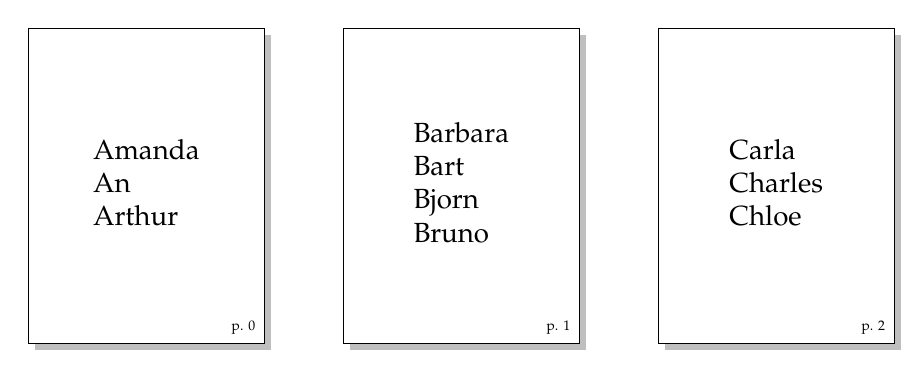
\begin{tikzpicture}
      \node[draw,minimum width=3cm,minimum height=4cm,fill=white,drop shadow] (page a) {
        \begin{tabular}{l}
          Amanda \\
          An \\
          Arthur
        \end{tabular}
      };
      \node[draw,minimum width=3cm,minimum height=4cm,fill=white,drop shadow] at (4,0) (page b) {
        \begin{tabular}{l}
          Barbara \\
          Bart \\
          Bjorn \\
          Bruno \\
        \end{tabular}
      };
      \node[draw,minimum width=3cm,minimum height=4cm,fill=white,drop shadow] at (8,0) (page c) {
        \begin{tabular}{l}
          Carla \\
          Charles \\
          Chloe \\
        \end{tabular}
      };
      \node[anchor=south east,font=\tiny] at (page a.south east) {p. 0};
      \node[anchor=south east,font=\tiny] at (page b.south east) {p. 1};
      \node[anchor=south east,font=\tiny] at (page c.south east) {p. 2};
    \end{tikzpicture}
  \end{center}
\end{frame}

\begin{frame}
  \frametitle{Poging \#1: Code}
  \code[language=python]{dict1.py}
\end{frame}

\begin{frame}
  \frametitle{Verdeling}
  \begin{center}
    \includegraphics[width=5cm]{prefix1.png}
  \end{center}
  \begin{center}
    \begin{tabular}{cc@{\hspace{1cm}}cc}
      \bfseries letter & \bfseries \# namen & \bfseries letter & \bfseries \# namen \\
      \toprule
      m & 174 & c & 118 \\
      a & 161 & g & 116 \\
      j & 147 & r & 108 \\
      s & 138 & d & 89 \\
      l & 125 & e & 88 \\
      b & 120 & t & 87
    \end{tabular}
  \end{center}
% [('q', 3), ('x', 3), ('z', 9), ('u', 10), ('y', 12), ('o', 22), ('i', 32), ('v', 45), ('w', 57), ('n', 69), ('p', 70), ('k', 72), ('h', 79), ('f', 87), ('t', 87), ('e', 88), ('d', 89), ('r', 108), ('g', 116), ('c', 118), ('b', 120), ('l', 125), ('s', 138), ('j', 147), ('a', 161), ('m', 174)]
\end{frame}

\begin{frame}
  \frametitle{Poging \#1: Evaluatie}
  \structure{Voordelen}
  \begin{itemize}
    \item Alfabetische zoektocht beperkt zich tot namen met zelfde eerste letter
    \item Gemiddeld 26$\times$ minder namen om alfabetisch te doorzoeken
  \end{itemize}
  \vskip5mm
  \structure{Probleem}
  \begin{itemize}
    \item Een pagina kan nog steeds veel woorden bevatten
    \item Kunnen we geen extra pagina's toevoegen?
  \end{itemize}
\end{frame}

\begin{frame}
  \frametitle{Poging \#2}
  \begin{itemize}
    \item Ons niet beperken tot enkel eerste letter
    \item Paginanummer afleiden uit 2 eerste letters
  \end{itemize}
  \begin{center}
    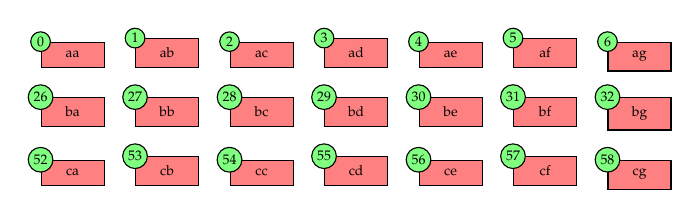
\begin{tikzpicture}
      \foreach[count=\xi,evaluate={\xi*0.75} as \px] \x in {a,b,c} {
        \foreach[count=\yi,evaluate={\yi*1.2} as \py,evaluate={int((\xi-1)*26+\yi-1)} as \p] \y in {a,b,c,d,e,f,g} {
          \node[draw,fill=red!50,font=\tiny,anchor=base,minimum width=.8cm] (c) at (\py,-\px) {\x\y};
          \node[draw,circle,font=\tiny,inner sep=1pt,fill=green!50] at (c.north west) {\p};
        }
      }
    \end{tikzpicture}
  \end{center}
  \vskip2mm
  \structure{Voorbeeld}
  \begin{itemize}
    \item \textbf{Aa}ron op pagina 0
    \item \textbf{Ab}raham op pagina 1
    \item \textbf{Ac}hiel op pagina 2
  \end{itemize}
\end{frame}

\begin{frame}
  \frametitle{Poging \#2: Code}
  \code[language=python,font=\small,width=.95\linewidth]{dict2.py}
\end{frame}

\begin{frame}
  \frametitle{Poging \#2: Evaluatie}
  \structure{Voordelen}
  \begin{itemize}
    \item We hoeven enkel alfabetisch te zoeken binnen woorden met dezelfde 2 beginletters
    \item $26^2 = 676\times$ minder woorden om alfabetisch in te zoeken
  \end{itemize}
  \vskip5mm
  \structure{Mogelijke Verbetering}
  \begin{itemize}
    \item Waarom niet uitbreiden naar 3, 4, 5, \dots\ beginletters?
  \end{itemize}
\end{frame}

\begin{frame}
  \frametitle{Extrapoleren}
  \begin{center}
    \begin{tabular}{cc}
      \bfseries \#letters & \bfseries \#pagina's \\
      \toprule
      1 & 26 \\
      2 & 676 \\
      3 & \SI{17576}{} \\
      4 & \SI{456976}{} \\
      5 & \SI{11881376}{} \\
    \end{tabular}
  \end{center}
  \begin{itemize}
    \item Hoe meer letters hoe beter
    \item Uiteindelijk nog maar max.~1 woord per pagina
    \item We kunnen elk woord in \'e\'en stap terugvinden!
  \end{itemize}
\end{frame}

\begin{frame}
  \frametitle{Nadeel}
  \begin{itemize}
    \item Veel pagina's vergt veel geheugen
    \item Namenlijst van 12 miljoen pagina's onhandig
    \item Evenwicht zoeken
    \item Bv. stel dat er \SI{100000} namen zijn
    \item Alfabetisch opzoeken in lijst van max.\ 10 namen
    \item Drie letters gebruiken lijkt best
  \end{itemize}
  \begin{center}
    \begin{tabular}{ccc}
      \bfseries\#letters & \bfseries\#pagina's & \bfseries\#namen/pagina \\
      \toprule
      1 & 26 & $\pm$4000 \\
      2 & 676 & $\pm$150 \\
      \color{red} 3 & \color{red} \SI{17576}{} & \color{red} $\pm$ 6 \\
      4 & \SI{456976}{} & $\pm$ 0.21 \\
      5 & \SI{11881376}{} & $\pm$ 0.008 \\
    \end{tabular}
  \end{center}
\end{frame}

\begin{frame}
  \frametitle{Nog Meer Nadelen}
  \structure{Andere Types Objecten}
  \begin{itemize}
    \item Deze techniek werkt enkel op strings
    \item Wat met andere objecten? Geen naamlijst maar
          \begin{itemize}
            \item Lijst getallen
            \item Lijst datums
            \item \dots
          \end{itemize}
  \end{itemize}
  \vskip5mm
  \structure{Onbekend Aantal}
  \begin{itemize}
    \item In geval van ons voorbeeld is aantal op voorhand gekend
    \item Wat als niet op voorhand geweten hoeveel namen?
          \begin{itemize}
            \item Hoe weten we hoeveel letters we moeten gebruiken?
          \end{itemize}
    \item Wat als het aantal namen kan veranderen?
          \begin{itemize}
            \item Het aantal letters moet telkens aangepast worden
          \end{itemize}
  \end{itemize}
\end{frame}

\begin{frame}
  \frametitle{Veralgemenen Berekening Paginanummer}
  \begin{itemize}
    \item Paginaberekening gebeurt nu op basis van $n$ eerste letters
    \item Is het belangrijk dat dit exact zo gebeurt?
    \item Een willekeurige berekening voldoet
    \item We noemen paginaberekening \emph{hashing}
    \item We vergelijken een aantal hashfuncties
  \end{itemize}
\end{frame}

\begin{frame}
  \frametitle{Hashes}
  \vskip2mm
  \begin{overprint}
    \onslide<1>
    \begin{center}
      Eerste Letter
    \end{center}
    \onslide<2>
    \begin{center}
      Eerste Twee Letter
    \end{center}
    \onslide<3>
    \begin{center}
      Eerste Drie Letter
    \end{center}
    \onslide<4>
    \begin{center}
      Lengte
    \end{center}
    \onslide<5>
    \begin{center}
      Som Letters
    \end{center}
  \end{overprint}

  \begin{overprint}
    \onslide<1>
    \begin{center}
      \includegraphics[width=6cm]{prefix1.png}
    \end{center}
    \onslide<2>
    \begin{center}
      \includegraphics[width=6cm]{prefix2.png}
    \end{center}
    \onslide<3>
    \begin{center}
      \includegraphics[width=6cm]{prefix3.png}
    \end{center}
    \onslide<4>
    \begin{center}
      \includegraphics[width=6cm]{length.png}
    \end{center}
    \onslide<5>
    \begin{center}
      \includegraphics[width=6cm]{sum.png}
    \end{center}
  \end{overprint}
  \vskip2mm
  \begin{overprint}
    \onslide<1>
    \begin{center}
      \begin{tabular}{cccccc}
        \bfseries Aaa & \bfseries Aab & \bfseries Aac & \dots & \bfseries Aar & \dots \\
        \toprule
         & & & & Aaron \\
      \end{tabular}
    \end{center}

    \onslide<2>
    \begin{center}
      \begin{tabular}{cccc}
        \bfseries A & \bfseries B & \bfseries C & \dots \\
        \toprule
        An & Bart & Carl \\
        Albert & Bert & Christine \\
        Alex & Bruce & Claude \\
      \end{tabular}
    \end{center}

    \onslide<3>
    \begin{center}
      \begin{tabular}{cccc}
        \bfseries Aa & \bfseries Ab & \bfseries Ac & \dots \\
        \toprule
        Aaron & Abel & Achiel \\
         & Abraham &  \\
      \end{tabular}
    \end{center}

    \onslide<4>
    \begin{center}
      \begin{tabular}{ccccc}
        \bfseries 1 & \bfseries 2 & \bfseries 3 & \bfseries 4 & \dots \\
        \toprule
         & Jo & Els & Koen \\
         & Al & Luc & Jens \\
         & An & Jef & Ines \\
         &    & Ken & Lars \\
      \end{tabular}
    \end{center}

    \onslide<5>
  \end{overprint}
\end{frame}

\begin{frame}
  \frametitle{Evaluatie Hashfuncties}
  \begin{itemize}
    \item Welke is de beste hashfunctie?
    \item Wat kenmerkt een hashfunctie?
          \begin{itemize}
            \item Wat zijn goede kenmerken?
            \item Wat zijn slechte kenmerken?
          \end{itemize}
  \end{itemize}
\end{frame}

\begin{frame}
  \frametitle{Aspect \#1: Bereik}
  \begin{center}
    \begin{tabular}{lc}
      \bfseries Algoritme & \bfseries Aantal pagina's \\
      \toprule
      Eerste letter & 26 \\
      Twee eerste letters & $26^2 = 676$ \\
      Drie eerste letters & $26^3 = 17576$ \\
      Lengte & 15 \\
      Som letters & 300 \\
    \end{tabular}
  \end{center}
  \begin{center}
    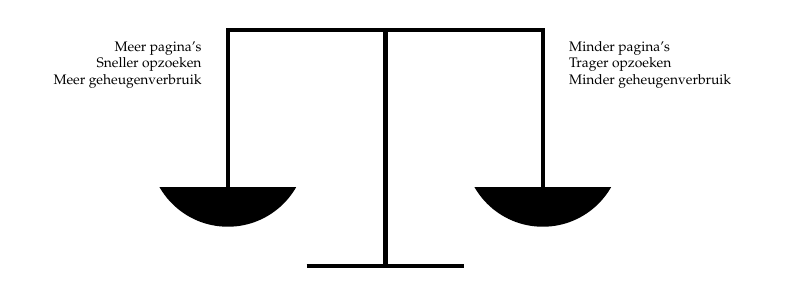
\begin{tikzpicture}
      \draw[ultra thick] (0,1) -- (0,4);
      \draw[ultra thick] (-1,1) -- (1,1);
      \draw[ultra thick] (-2,2) -- (-2,4) -- (2,4) -- (2,2);
      
      \begin{scope}
        \path[clip] (-3,1) rectangle (-1,2);
        \path[fill=black] (-2,2.5) circle [radius=1cm];
      \end{scope}

      \begin{scope}
        \path[clip] (3,1) rectangle (1,2);
        \path[fill=black] (2,2.5) circle [radius=1cm];
      \end{scope}

      \node[anchor=north east,font=\tiny] at (-2,4) {
        \begin{tabular}{r}
          Meer pagina's \\
          Sneller opzoeken \\
          Meer geheugenverbruik \\
        \end{tabular}
      };
      \node[anchor=north west,font=\tiny] at (2,4) {
        \begin{tabular}{l}
          Minder pagina's \\
          Trager opzoeken \\
          Minder geheugenverbruik \\
        \end{tabular}
      };
    \end{tikzpicture}
  \end{center}
\end{frame}

\begin{frame}
  \frametitle{Bereik Aanpassen}
  \begin{itemize}
    \item Een hash met een te groot bereik kan gemakkelijk ingeperkt worden
    \item Stel hash geen aanleiding tot 1 miljoen pagina's
    \item We willen er maar 100
    \item Oplossing: we bekijken enkel de 2 laatste cijfers
  \end{itemize}
  \begin{center}
    \begin{tabular}{r@{$\;\rightarrow\;$}l}
      \bfseries Hash & \bfseries Aanpassing \\
      \toprule
      0 & 0 \\
      1 & 1 \\
      531 & 31 \\
      46716156 & 56 \\
    \end{tabular}
  \end{center}
\end{frame}

\begin{frame}
  \frametitle{Bereik Hash: Conclusie}
  \begin{itemize}
    \item Een te groot bereik kan ingeperkt worden
    \item Een te klein bereik kan niet uitgebreid worden
    \item Hashes met groot bereik zijn \emph{altijd} beter
  \end{itemize}
  \begin{center}
    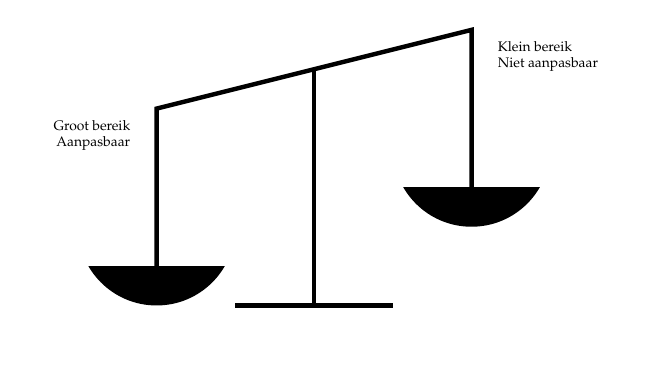
\begin{tikzpicture}
      \draw[ultra thick] (0,1) -- (0,4);
      \draw[ultra thick] (-1,1) -- (1,1);
      \draw[ultra thick] (-2,1.5) -- (-2,3.5) -- (2,4.5) -- (2,2.5);
      
      \begin{scope}[yshift=-0.5cm]
        \path[clip] (-3,1) rectangle (-1,2);
        \path[fill=black] (-2,2.5) circle [radius=1cm];
      \end{scope}

      \begin{scope}[yshift=0.5cm]
        \path[clip] (3,1) rectangle (1,2);
        \path[fill=black] (2,2.5) circle [radius=1cm];
      \end{scope}

      \node[anchor=north east,font=\tiny] at (-2,3.5) {
        \begin{tabular}{r}
          Groot bereik \\
          Aanpasbaar \\
        \end{tabular}
      };
      \node[anchor=north west,font=\tiny] at (2,4.5) {
        \begin{tabular}{l}
          Klein bereik \\
          Niet aanpasbaar \\
        \end{tabular}
      };
    \end{tikzpicture}
  \end{center}
\end{frame}

\begin{frame}
  \frametitle{Aspect \#2: Verdeling}
  \begin{itemize}
    \item Verdeling over pagina's niet uniform
          \begin{itemize}
            \item Veel meer namen beginnend met M dan met X
            \item Veel meer namen van 6 lang dan van 15 lang
          \end{itemize}
    \item Zoeken naar hashfunctie met uniforme verdeling
    \item Hoe uniformer, hoe beter
  \end{itemize}
  \begin{center}
    \begin{tabular}{cc}
      \includegraphics[width=4cm]{uneven.png}
      &
      \includegraphics[width=4cm]{uniform.png} \\
      niet uniform & uniform
    \end{tabular}
  \end{center}
\end{frame}

\begin{frame}
  \frametitle{Samenvatting}
  \begin{itemize}
    \item Een hashfunctie associeert een getal met een object
    \item Het bereik moet zo groot mogelijk zijn
    \item Verdeling moet zo uniform mogelijk zijn
    \item Ideale wereld: \'e\'en unieke hash per object
  \end{itemize}
\end{frame}

\begin{frame}
  \frametitle{Namenlijst Met Hashing}
  \begin{center}
    \begin{tabular}{ccc}
      \bfseries Naam & \bfseries Hash & \visible<3>{\bfseries Pagina} \\
      \toprule
      Jan     & 3497913\alert<2>5 & \visible<3>5 \\
      Nicolas & 6764651\alert<2>3 & \visible<3>2 \\
      Eva     & 1346465\alert<2>4 & \visible<3>4 \\
      Stefaan & 5762135\alert<2>0 & \visible<3>0 \\
      Geert   & 1546513\alert<2>7 & \visible<3>7 \\
    \end{tabular}
  \end{center}
  \begin{itemize}
    \item Slechts 5 namen
    \item<2-> We beschouwen enkel laatste cijfer van hash
    \item<3> In totaal 10 pagina's
  \end{itemize}
\end{frame}

\begin{frame}
  \frametitle{Namenlijst Met Hashing}
  \begin{center}
    \begin{tabular}{ccc}
      \bfseries Naam & \bfseries Hash & \visible<3>{\bfseries Pagina} \\
      \toprule
      Jan     & 349791\alert<2>{35} & \visible<3>{35} \\
      Nicolas & 676465\alert<2>{13} & \visible<3>{12} \\
      Eva     & 134646\alert<2>{54} & \visible<3>{54} \\
      Stefaan & 576213\alert<2>{50} & \visible<3>{50} \\
      Geert   & 154651\alert<2>{37} & \visible<3>{37} \\
      Frank   & 462323\alert<2>{53} & \visible<3>{53} \\
      Victor  & 540324\alert<2>{97} & \visible<3>{97} \\
      \vdots  & \vdots              & \visible<3>{\vdots} \\
    \end{tabular}
  \end{center}
  \begin{itemize}
    \item Er komen namen bij, stel 100 in totaal
    \item Gemiddeld 10 namen per pagina
    \item<2-> We gooien de 10 pagina's weg en beginnen opnieuw
    \item<2-> We beschouwen de 2 laatste cijfer van hash
    \item<3> We verkrijgen 100 pagina's met gemiddeld 1 naam/pagina
  \end{itemize}
\end{frame}

\begin{frame}
  \frametitle{Werking Set: Initialisatie}
  \begin{itemize}
    \item Pagina heet nu bucket
    \item Een bucket is een lijst
    \item Initieel beginnen met bv.~8 buckets
    \item 3 laatste bits van hashes bepalen bucket
  \end{itemize}
  \code[language=python,font=\small,width=.9\linewidth]{set-init.py}
\end{frame}

\begin{frame}
  \frametitle{Werking Set: Toevoegen Element}
  \begin{itemize}
    \item Nieuwe elementen worden gehasht
    \item Laatste $N$ digits bepalen index
  \end{itemize}
  \code[language=python,font=\small,width=.9\linewidth]{set-add.py}
\end{frame}

\begin{frame}
  \frametitle{Werking Set: Opzoeken Element}
  \begin{itemize}
    \item Element wordt gehasht
    \item $N$ laatste bits bepalen bucket
    \item Er wordt gezocht in die bucket
  \end{itemize}
  \code[language=python,font=\small,width=.9\linewidth]{set-member.py}
\end{frame}

\begin{frame}
  \frametitle{Werking Set: Herdistributie}
  \begin{itemize}
    \item Na een tijd te veel elementen per bucket
    \item Extra buckets aanmaken
  \end{itemize}
  \code[language=python,font=\scriptsize,width=.9\linewidth]{set-rehash.py}
\end{frame}

\begin{frame}
  \frametitle{Vereisten}
  \begin{itemize}
    \item Een set steunt op 2 operaties op zijn items
    \item Elementen moeten gehasht kunnen worden (\texttt{hash(x)})
          \begin{itemize}
            \item \texttt{\_\_hash\_\_} implementeren
          \end{itemize}
    \item Elementen moeten vergeleken kunnen worden (\texttt{x == y})
          \begin{itemize}
            \item \texttt{\_\_eq\_\_} implementeren
          \end{itemize}
    \item Belangrijk!
          \vskip4mm
          \begin{center} \alert{\fbox{Gelijke elementen moeten gelijke hashes hebben}} \end{center}
  \end{itemize}
\end{frame}

\begin{frame}
  \frametitle{Voorbeeld}
  \code[language=python,font=\small]{hash.py}
\end{frame}

\begin{frame}
  \frametitle{Probleem Met Mutability}
  \begin{itemize}
    \item Ik maak \texttt{t = Time(0, 0, 0)} aan
    \item Ik steek \texttt{t} in set
    \item Set hasht en steekt die in bucket 0
    \item Ik wijzig \texttt{t}: \texttt{t.s += 1}
    \item Ik vraag aan set of \texttt{t} erin steekt
    \item Set hasht en gaat zoeken in bucket 1
    \item Set vindt \texttt{t} niet
  \end{itemize}
\end{frame}

\begin{frame}
  \frametitle{Immutable Keys}
  \begin{itemize}
    \item Enkel onwijzigbare objecten gebruiken in sets/dicts
    \item Wijzigbare standaardklassen implementeren \texttt{\_\_hash\_\_} niet
          \begin{itemize}
            \item lists kan men niet steken in sets
            \item sets kan men niet steken in sets
            \item \dots
          \end{itemize}
    \item Python biedt onwijzigbare varianten
          \begin{itemize}
            \item Onwijzigbare list: tuple
            \item Onwijzigbare set: frozenset
          \end{itemize}
  \end{itemize}
\end{frame}

\end{document}



%%% Local Variables: 
%%% mode: latex
%%% TeX-master: t
%%% End: 
